\documentclass{beamer}
\usetheme{Frankfurt}

\usepackage{amsmath}
\usepackage{graphicx}

\title{A Markov Chains Application To Stock Markets}
\author{Federico Camerota}
\date{}

\begin{document}
	\maketitle
	\section{Model formulation}
	
	\begin{frame}{Main idea}
	\begin{itemize}
		\item We aim to use Markov Chains (MC) to model the state of a stock market and
		the price of the single stocks in it. The behaviors are studied on a daily basis so we use
		discrete time MCs.\\
		\vspace{10pt}
		\item The purpose is to study the ability of predicting future trends of stock prices of such a model and to 
		investigate if the information obtained by simulating the stock market with the model can be used in a 
		portfolio selection strategy with good results.
	\end{itemize}
	\end{frame}
	
	
	\begin{frame}{Market chain}
	\begin{itemize}
		\item For the market we consider two possible states: \textbf{\textit{bad}} and \textbf{\textit{good}}.
		\item A transition to the state \textit{good} is defined as an increase in the overall
			  market value. While a transition to the \textit{bad} state is defined as a decrease
			  of such quantity.
		\item So the MC describing the market is characterized by the following transition matrix\\
				\vspace{2pt}
				\begin{center}
				\begin{tabular}{c|c|c|}
					\phantom{good} & \textit{bad}  & \textit{good}\\
					\hline
					\textit{bad}   & $1 - p_{b2g}$ & $p_{b2g}$\\
					\hline
					\textit{good}  & $p_{g2b}$     & $1 - p_{g2b}$\\
					\hline
				\end{tabular}
				\end{center}	
	\end{itemize}
	\end{frame}

	\begin{frame}{Stock chain}
	\begin{itemize}
		\item We consider as initial state the last observed stock price and assume that the daily price variation is a decrease or an increase by a fixed $\delta$ that depends on the 
			  state of the market.
		\item The market state influences both the daily variation $delta$ and the probability of an increase/decrease. However these probabilities are assumed to be independent of the
		      current stock price.
	\end{itemize}
	\end{frame}

	\begin{frame}{Stock chain}
	\begin{itemize}
		\item We end up with a complex transition matrix, however, due to the previous assumptions, the stock MC can be described by the following parameters:	
			\begin{center}
				\begin{enumerate}
					\item $\delta_{g,m}$ and $\delta_{b,m}$ that describe the daily price variation of stock $m$ when the market is in good and bad state.
					\item $p_{g,m}$ and $p_{b,m}$ that are the probabilities of an increase in the price of stock $m$ when the market is in good and bad state.
				\end{enumerate}
			\end{center}
	\end{itemize}
	\end{frame}

	\begin{frame}{Comments and possible extensions}
		\begin{itemize}
			\item The definition of market states is quite naive, this could be improved by considering trends and the amount of variation in the market value.
			\item Another underlying assumption is that the stock chains are independent. The model could be improved by considering correlations, for example clustering stocks with
				  similar time evolution and then simulating a common trajectory for the cluster and the discrepancy from it for each stock in the cluster.
			\item In the stock chain the daily variation is kept fixed, an extension of the model that has been explored is the usage of a proposal distribution whose parameters are 
				  estimated from the data. We tested normal distributed daily variations.
		\end{itemize}
	\end{frame}
	
	\section{Data and parameter estimation}
		\begin{frame}{Data Set}
		\begin{itemize}
			\item The data used has been obtained from \hyperlink{https://www.kaggle.com/dgawlik/nyse\#securities.csv}{Kaggle} and are daily prices of stocks in the New York Stock Exchange (NYSE).
			\item From the data we define the overall market price as the sum of all stock prices.
		\end{itemize}
		\end{frame}
	
	\begin{frame}{Data model}
	\begin{itemize}
		\item To estimate the parameters of the model we consider the time series of ups and downs is the prices of both the market and the stocks. Encoding an up with $1$ and a down with $0$.
		\item  Under the assumptions of the model the market trend series is a sequence of Bernoulli random variables with parameter that depends on the previous observation.
							$$M_t \sim \text{Bernoulli}(p_t)$$
					 where $p_t$ is equal to $p_{b2g}$ if $M_{t-1} = 0$ and $1 - p{g2b}$ otherwise. 
		
	\end{itemize}
	\end{frame}

	\begin{frame}{Data model}
	\begin{itemize}
		\item The stock trend series instead turn out to be independent Bernoulli variables with parameter that depends on the current market state
				$$S_{t,m} \sim \text{Bernoulli}(p_{t,m})$$
			  where $p_{t,m}$ is equal to $p_{g,m}$ if $M_t = 1$ and $p_{b,m}$ otherwise.
	\end{itemize}
	\end{frame}
	
	\begin{frame}{Parameter Estimation}
	\begin{itemize}
		\item Considering the market trend series and a single stock trend series, the parameters in the two MCs can be estimated through maximum likelihood quite easily.
		\item The estimators found this way can be extended to all the stocks considered due to the hypothesis that the stock chains are independent.
		\item In fact, the estimators for the market chain depend only on the market behavior while the estimators for the stock chain depend only on the stock observed trends.
		\item For the $delta$ parameters in the stock chains we propose three different approaches:
			\begin{enumerate}
				\item Mean daily variations
				\item Median daily variations
				\item 10th percentile of daily variations
			\end{enumerate}
	\end{itemize}
	\end{frame}

	\begin{frame}{Comments and possible extensions}
	\begin{itemize}
		\item Another possible extension of the model could be the usage of \textbf{continuous time} MCs. However, since the available data is on a daily basis we consider it won't make
			  much sense in this framework. Given more frequent data this approach could yield a better model.
		\item In the parameter estimation we give the same importance to all the observations considered, we could instead use different weight profiles for each stock in order to 
			  exploit the information present in the time series and have better parameter estimates. On the proposed data model the usage of \textbf{weighted likelihood} seems a bit difficult
			  so this extension has not been studied.
	\end{itemize}
	\end{frame}

	\section{Computational experiments}
		\begin{frame}{Experiments}
		\begin{itemize}
			\item We propose two study cases to test our model. 
			\item The first experiment (\textit{portfolio selection}) consists in using the results of a fixed number of simulations ran using our model as data in a portfolio selection 
				  problem and compare its performance with respect to a portfolio obtained only using historical data.
	    	\item In the second experiment we study the ability of the model to predict future stock trajectories.
		\end{itemize}	
		\end{frame}

		\begin{frame}{Portfolio selection}
		\begin{itemize}
			\item As selection strategy we use the maximization of the \textit{Sharpe ratio} defined as the ratio of the expected return and variance.
			\item To solve the problem we use standard numerical methods provided in the $scipy$ module. We also tested the usage of an heuristic method to solve the problem but the runtime is
		          considerably higher and results don't seem to be superior.
			\item The strategy based on historical data uses expected returns and variances estimated over the last 200 days while the strategy based on simulations uses expected returns and
			  	  variance of the simulated return for a given time horizon.
			\item The experiment has been conducted using three different time horizons: 7, 15 and 30 days.
		\end{itemize}
		\end{frame}
	
		\begin{frame}{Portfolio selection results}
		\begin{itemize}
			\item As a benchmark we consider a strategy that invests the same amount of capital on each stock in the market.
			\item The best setting is the one using the mean as $\delta$ and a re-calibration period of 15 days.
			\item We tested the method with the above setting on a sample of 30 days with a time horizon of 120 days.
		\end{itemize}
			\begin{center}
				\begin{tabular}{|c|c|c|c|c|}
					\hline
					Method & Avg. Return & Return std & Min return & Max return\\
					\hline
					\hline
					Naive & 0.00791 & 0.03271 & -0.1562 & 0.1601\\
					\hline
					StockMC & 0.01022 & 0.05621 & -0.1923 & 0.1826\\
					\hline
					StockMC2 & 0.006692 & 0.09676 & -0.4221 & 0.3298\\
					\hline
				\end{tabular}
			\end{center}
		\end{frame}
	
		\begin{frame}{Portfolio selection results}
		\begin{itemize}
			\item The variability of the obtained returns is quite high.
			\item The overall return is not much better than the one obtained with the benchmark.
			\item The method doesn't seem to improve on a strategy that only uses time series data.
		\end{itemize}
		\end{frame}
	
		\begin{frame}{Trajectories experiment}
		\begin{itemize}
			\item In this problem the best setting appears to be the one using the mean as $\delta$ and a window of 7 days.
			\item Using the above setting we tested the ability of the method to predict the price trajectories of a sample of stocks.
		\end{itemize}	
			 \begin{center}
			 	\begin{tabular}{|c|c|c|c|c|}
			 		\hline
			 		Qty. & Average & Std. Deviation & Minimum & Maximum\\
			 		\hline
			 		\hline
			 		MSE & 6.0319   & 28.3576        & 0.00055 & 803.9234\\
			 		\hline
			 	\end{tabular}
			 \end{center}
		\end{frame}	
	
	\begin{frame}{Trajectories experiment}
	\begin{itemize}
		\item The results show that the model is not able to predict properly future price trends.
		\item It appears that the evolution scheme used is too rigid and the average simulated trajectories tend to be quite flat.
	\end{itemize}
	\begin{figure}
	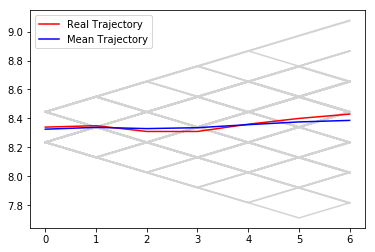
\includegraphics[width=0.5\textwidth]{../images/best_mse.png}%
	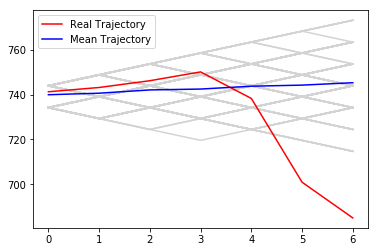
\includegraphics[width=0.5\textwidth]{../images/worst_mse.png}
	\caption{Best and worst case in terms of MSE}
	\end{figure}
	\end{frame}

	\begin{frame}{Conclusions}
	\begin{itemize}
		\item We conclude that the proposed model doesn't work properly in the studied problems.
		\item A possible improvement in the portfolio problem could be the use of a better selection strategy.
		\item In the trajectories problem the model should be able to be more flexible, this could be achieved by
			  using higher order MCs or some other strategy to take into account the price trends.
	\end{itemize}
	\end{frame}

\end{document}